\documentclass[14pt, letterpaper]{article}
\usepackage[utf8]{inputenc}
\usepackage[a4paper, total={6in, 8in}]{geometry}
\usepackage{listings}
\usepackage{enumitem}
\usepackage{graphicx}

\begin{document}
\include{mytitle}
 
\begin{titlepage}
	\begin{center}
	\fontsize{14pt}{14pt} \selectfont {College of Engineering Trivandrum}\\
	\vspace*{0.8cm}
	\vspace*{1.5cm}	
	\fontsize{18pt}{1cm}\selectfont\textbf{{Data Structures Lab}}\\
	\vspace*{0.8cm}
	\vspace*{1.5cm}
	
\includegraphics[width=2in]{images/cet emblem.jpg}\\
	\vspace*{2.5cm}
	\fontsize{14pt}{14pt} \selectfont{ Aishwarya A J}\\
	\vspace{0.2cm}
	\fontsize{14pt}{14pt} \selectfont{S3 CSE Roll No:6}\\
	\vspace*{0.2cm}
	\fontsize{14pt}{14pt} \selectfont{TVE19CS006}\\
	\vspace*{2cm}
	\fontsize{18pt}{1cm}\selectfont {Department Of Computer Science}\\
	\vspace{0.5cm}
		\fontsize{18pt}{18pt}\selectfont{November 24, 2020}
\end{center}
\end{titlepage}
\newpage
\tableofcontents
\newpage
\noindent

\includegraphics[width=0.5in]{images/cet emblem 1.jpg}
\hfill
  \textbf{ \huge{\underline{CSL 201-Data Structures Lab - Cycle 2 }}}
  \begin{center}
       \vspace{0.5 cm}
       \fontsize{18pt}{18pt}\textbf{Part-2}
  \end{center}
\section{Binary Search Tree}

\subsection{Problem}
Create a binary Search Tree with the following operations\\
a. Insert a new node\\
b. Inorder traversal\\
c. Preorder traversal\\
d. Postorder traversal\\
e. Delete a node
\subsection{Algorithm}
\hline 
\vspace{0.1cm}
\hspace{0.2 cm}Algorithm 1:Binary Search Tree Operations
\vspace{0.1cm}
\hline

\begin{lstlisting}[label={list:first}]
 Declare structure treeNode with data,treeNode*lc and treeNode*rc as members 
 
 START OF FUNCTION inorder(treeNode *root) 
 If(root!=NULL) 
    inorder(root->lc)
    Print root->data
    inorder(root->rc)
 End If
 END OF FUNCTION inorder
 
 START OF FUNCTION postorder(treeNode* node)
 If(node!=NULL)
    postorder(node->lc)
    postorder(node->rc)
    Print node->data
 End if
 END OF FUNCTION postorder
 
 START OF FUNCTION preorder(treeNode* node) 
 If(node!=NULL)
    Print node->data
    preorder(node->lc)
    preorder(node->rc)
 End if
 END OF FUNCTION preorder
   
 START OF FUNCTION insertIntoTree(treeNode* root, int data)
 /*Insert into the binary search tree node with value="data" and return the
 root of the tree*/
 If(root==NULL)
     Allocate memory for ptr
     ptr->data=data
     ptr->lc=NULL
     ptr->rc=NULL
     root=ptr
 Else
      If(root->data>data)
         root->lc=insertIntoTree(root->lc, data)
      Else if(root->data<data) 
         root->rc=insertIntoTree(root->rc, data)               
      End if     
 End if  
 Return root
 END OF FUNCTION insertIntoTree
 
 START OF FUNCTION  deleteFromTree(struct treeNode* root, int data) 
 //Delete from the BST node with value = "data" and then return root of the tree
 ptr=root
 flag=0
 While(ptr!=NULL and flag==0) do
     If (data<ptr->data) 
         parent=ptr
         ptr=ptr->lc
     Else if(data>ptr->data)
         parent=ptr
         ptr=ptr->rc
     Else set flag=1
     End if
 End While
 If(flag==0) Return root
 Else
    If(ptr->lc==NULL and ptr->rc==NULL)
         If(parent->lc==ptr)
              parent->lc=NULL
         Else 
              parent->rc=NULL
         End if
    Else if(ptr->lc && ptr->rc)
         ptr1=ptr->rc
         If(ptr1!=NULL)
            While(ptr1->lc!=NULL)
                 ptr1=ptr1->lc
            End while
         End if
         i=ptr1->data
         deleteFromTree(root,i)
         ptr->data=i
    Else
         If(parent->lc==ptr)
             If(ptr->lc==NULL)
                  parent->lc=ptr->rc
             Else 
                  parent->lc=ptr->lc
             End if
         Else if(parent->rc==ptr)
             If(ptr->lc==NULL)
                  parent->rc=ptr->rc
             Else 
                  parent->rc=ptr->lc
             End if
        End if
    End if
 End if
 Return root
 END OF FUNCTION deleteFromTree
   
 START OF MAIN FUNCTION
 root = NULL
 Input option opt
 While(opt!=6)
    Switch(opt){
        Case 1: Input data 
                root = insertIntoTree(root,data)
                break
        Case 2: Input data                   
                root = deleteFromTree(root,data)
                break
        Case 3: inorder(root)
                break
        Case 4: preorder(root)
                break
        Case 5: postorder(root)
                break
    End switch-case
    Input opt
 End while
 END OF MAIN FUNCTION  
   
\end{lstlisting}
\hline


\subsection{Code}

\begin{lstlisting}[language=C,showstringspaces=false]
#include <math.h>
#include <stdio.h>
#include <string.h>
#include <stdlib.h>
#include <assert.h>
#include <limits.h>
#include <stdbool.h>

typedef struct treeNode{
    int data;
    struct treeNode *lc;
    struct treeNode *rc;
}treeNode;

void inorder(treeNode *root) {
    if(root){
        inorder(root->lc);
        printf("%d ",root->data);
        inorder(root->rc);
        
    }
} 

void postorder(treeNode* node){ 
    if(node){
        postorder(node->lc);
        postorder(node->rc);
        printf("%d ",node->data);
    }
} 

void preorder(treeNode* node) { 
    if(node){
        printf("%d ",node->data);
        preorder(node->lc);
        preorder(node->rc);
    }
} 

treeNode* insertIntoTree(treeNode* root, int data){
    if(root==NULL){
        treeNode*ptr;
        ptr=malloc(sizeof(treeNode));
        ptr->data=data;
        ptr->lc=NULL;
        ptr->rc=NULL;
        root=ptr;
    }
    else{
            if(root->data>data){
                root->lc=insertIntoTree(root->lc, data);
            }
            else if(root->data<data) {
                root->rc=insertIntoTree(root->rc, data);                
            }
    }
    return root;
} 
  
treeNode* deleteFromTree(struct treeNode* root, int data) 
{ 
    treeNode *ptr=root,*parent;
    int flag=0;
    while(ptr!=NULL && flag==0){
        if (data<ptr->data) {
            parent=ptr;
            ptr=ptr->lc;
        }
        else if(data>ptr->data){
            parent=ptr;
            ptr=ptr->rc;
        }
        else flag=1;
    }
    if(flag==0) return root;
    else{
        if(ptr->lc==NULL && ptr->rc==NULL){
            if(parent->lc==ptr)
               parent->lc=NULL;
            else 
               parent->rc=NULL;
        }
        else if(ptr->lc && ptr->rc){
            treeNode*ptr1=ptr->rc;
            if(ptr1){
                while(ptr1->lc)
                  ptr1=ptr1->lc;
            }
            int i=ptr1->data;
            deleteFromTree(root,i);
            ptr->data=i;
        }
        else{
            if(parent->lc==ptr){
                if(ptr->lc==NULL)
                   parent->lc=ptr->rc;
                else 
                   parent->lc=ptr->lc;
            }
            else if(parent->rc==ptr){
                if(ptr->lc==NULL)
                   parent->rc=ptr->rc;
                else 
                   parent->rc=ptr->lc;
            }
        }
        return root;
    }
} 
int main(){
    treeNode* root;
    root = NULL;
    int opt,data;
    do{
        scanf("%d",&opt);
        switch(opt){
            case 1: scanf("%d",&data);
                    root = insertIntoTree(root,data);
                    break;
            case 2: scanf("%d",&data);                   
                    root = deleteFromTree(root,data);
                    break;
            case 3: inorder(root);
                    printf("\n");
                    break;
            case 4: preorder(root);
                    printf("\n");
                    break;
            case 5: postorder(root);
                    printf("\n");
                    break;
        }
    }while(opt != 6);
    return 0;
}
\end{lstlisting}
\subsection{Sample output}
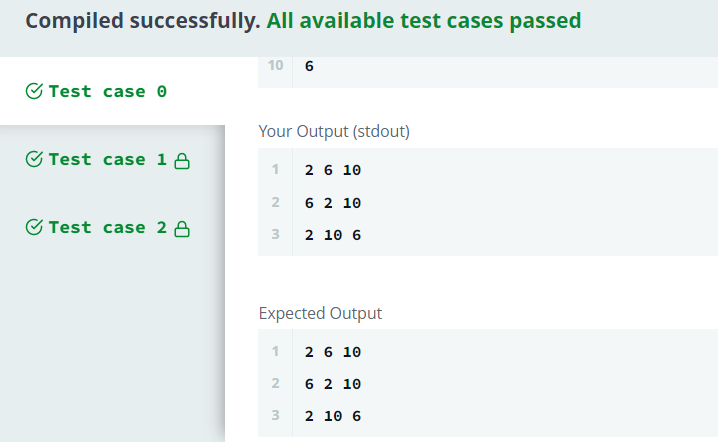
\includegraphics[width=\textwidth]{images/bst1.png}\\ \\
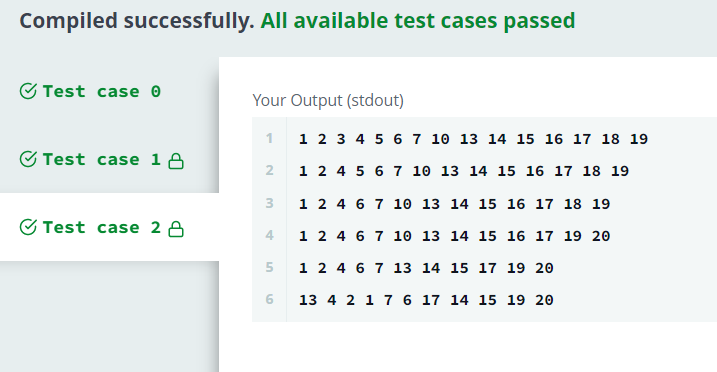
\includegraphics[width=\textwidth]{images/bst2.png}
\subsection{Result}
Program submitted and executed successfully in HackerRank Platform via user id\\ aishwaryaaj2002
\newpage
\section{Graphs}

\subsection{Problem}
Represent any given graph and\\
a. Compute adjacency list, adjacency matrix.\\
b. Perform a depth first search\\
c. Perform a breadth first search
\subsection{Adjacency List and Adjacency Matrix}
\subsubsection{Algorithm-Adjacency List}
\hline 
\vspace{0.1cm}
\hspace{0.5cm}Algorithm 2.a.1 :Adjacency List
\vspace{0.1cm}
\hline

\begin{lstlisting}[label={list:first}]
  Declare self-referential structure AdjacencyList with value and link as
  members.Declare array AdjacencyList g[size] with size =10
  
  START OF FUNCTION insert_to_graph(AdjacencyList * g,int parent,int value)
  ptr=g[parent]
  g[parent].value=parent
  Allocate memory for node
  node->value=value
  node->link=NULL
  While(ptr->link!=NULL)
     ptr=ptr->link
  End while     
  ptr->link=node
  END OF FUNCITON insert_to_graph
  
  START OF FUNCTION delete_from_graph(AdjacencyList * g,int value)
  Set flag=0
  If((g+value)->link!=NULL)
     (g+value)->link=NULL
     flag=1
  EndIf
  For i from 0 to size-1
     If(i!=value)
         ptr=g+i
         While(ptr->link!=NULL and ptr->value!=value)
             p=ptr
             ptr=ptr->link
         End While
         If(ptr->value==value)
             p->link=ptr->link
             flag=1
         EndIf
     EndIf
  End For
  If(flag==0)
     Print "Node does not exist !"
  EndIf
  END OF FUNCTION delete_from_graph

  START OF FUNCTION print_graph(AdjacencyList * g)
  Set flag=0
  ptr=(g+i)
  For i from 0 to size-1
    If((g+i)->link!=NULL)
        flag=1
        ptr=(g+i)
        Print "i ->"
        While(ptr->link!=NULL)
            Print ptr->link->value
            ptr=ptr->link
        EndWhile    
    EndIf
  End For
  If(flag==0)
      Print "Graph Empty !"
  EndIf
  END OF FUNCTION print_graph
  
  START OF MAIN FUNCTION
  Allocate memory for g
  g->link=NULL
  While(1)
    Input choice
    Switch(choice){
        Case 1: Input parent and value for insertion 
                insert_to_graph(g, parent, value) 
                break
        Case 2: Input value                   
                delete_from_graph(g,value)
                break
        Case 3: print_graph(g)
                break
        Case 4: return 0
    End switch-case
  End while
  END OF MAIN FUNCTION 
\end{lstlisting}
\hline


\subsubsection{Code-Adjacency List}
\begin{lstlisting}[language=C,showstringspaces=false]
#include <math.h>
#include <stdio.h>
#include <string.h>
#include <stdlib.h>
#include <assert.h>
#include <limits.h>
#include <stdbool.h>
typedef struct AdjacencyList
{
    int value;
    struct AdjacencyList*link;
}AdjacencyList;
AdjacencyList g[10];
void insert_to_graph(AdjacencyList * g,int parent,int value)
{
    AdjacencyList*ptr=g+parent,*node;
    g[parent].value=parent;
    node=(AdjacencyList*)malloc(sizeof(AdjacencyList));
    node->value=value;
    node->link=NULL;
    while(ptr->link!=NULL)
       ptr=ptr->link;
    ptr->link=node;
}

void delete_from_graph(AdjacencyList * g,int value)
{
   AdjacencyList*ptr,*p;
   int flag=0;
   if((g+value)->link){
   (g+value)->link=NULL;
   flag=1;
   }
   for(int i=0;i<10;i++){
     if(i!=value){
          ptr=g+i;
          while(ptr->link && ptr->value!=value){
              p=ptr;
             ptr=ptr->link;
          }
          if(ptr->value==value){
             p->link=ptr->link;
             flag=1;
          }
      }
   }
   if(flag==0){
       printf("Node %d does not exist !\n",value);
   }

}

void print_graph(AdjacencyList * g)
{
    int i,flag=0;
    AdjacencyList*ptr=(g+i);
    for(i=0;i<10;i++){
        if((g+i)->link){
            flag=1;
            AdjacencyList*ptr=(g+i);
            printf("%d ->",i);
            while(ptr->link){
              printf(" %d",ptr->link->value);
              ptr=ptr->link;
            }
            printf("\n");
        }
    }
    if(flag==0)
      printf("Graph Empty !\n");
}

int main() {
    AdjacencyList * g = (AdjacencyList *)malloc(sizeof(AdjacencyList)*10);
    g->link=NULL;
    while(1)
    {
        int choice;
        scanf("%d",&choice);
        switch(choice)
        {
            case 1:
            {
                int parent,value;
                scanf("%d %d",&parent,&value);
                insert_to_graph(g,parent,value);
            }
            break;

            case 2:
            {
                int value;
                scanf("%d",&value);
                delete_from_graph(g,value);
            }
            break;

            case 3:
            {
                print_graph(g);
            }
            break;

            case 4:
            {
                return 0;
            }
        }
    }
    return 0;
}

\end{lstlisting}

\subsubsection{Sample output}
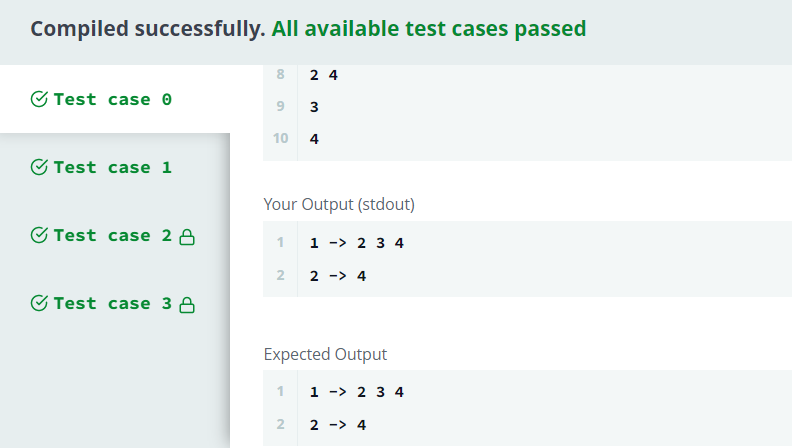
\includegraphics[width=5in]{images/adlist.png}\\ \\
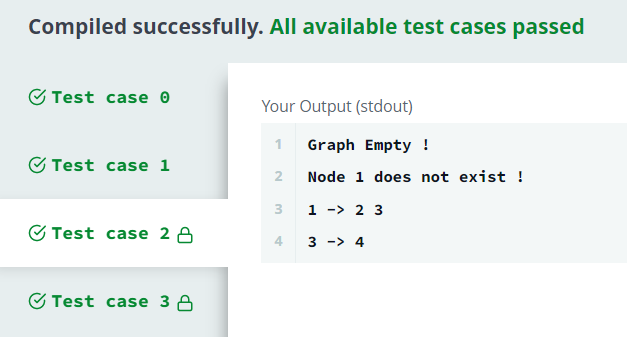
\includegraphics[width=5in]{images/adlist2.png}
\subsubsection{Algorithm-Adjacency Matrix}
\hline 
\vspace{0.1cm}
\hspace{0.5cm}Algorithm 2.a.2 :Adjacency Matrix
\vspace{0.1cm}
\hline

\begin{lstlisting}[label={list:first}]
  Declare a structure AdjacencyMatrix with mat[size][size] as member
  with size =10
  
  START OF FUNCTION insert_to_graph(AdjacencyMatrix*g,int parent,int value)
    g->mat[parent][value] =1
  END OF FUNCITON insert_to_graph
  
  START OF FUNCTION delete_from_graph(AdjacencyMatrix * g,int value)
  Set flag=0
  For i from 0 to size-1
     If(g->mat[value][i]==1)
        g->mat[value][i]=0
        flag=1
     Else If(g->mat[i][value]==1)
        g->mat[i][value]=0
        flag=1
     EndIf
  End For
  If(flag==0)
     Print "Node does not exist !"
  EndIf
  END OF FUNCTION delete_from_graph

  START OF FUNCTION print_graph(AdjacencyMatrix * g)
  Set n=-1,count=0,flag=0
  For i from 0 to size-1
    For i from 0 to size-1
        If(g->mat[i][j]==1)
            If(i==n)
                Print j
            Else
                If(count!=0)
                    Print "\n"
                EndIf
                Print i,j
                n=i
                count=count+1
            EndIf
            flag=1
       EndIf
    End For    
  End For
  If(flag==0)
      Print "Graph Empty !"
  EndIf
  END OF FUNCTION print_graph
  
  START OF MAIN FUNCTION
  Allocate memory for g
  While(1)
    Input choice
    Switch(choice){
        Case 1: Input parent and value for insertion 
                insert_to_graph(g, parent, value) 
                break
        Case 2: Input value                   
                delete_from_graph(g,value)
                break
        Case 3: print_graph(g)
                break
        Case 4: return 0
    End switch-case
  End while
  END OF MAIN FUNCTION 
\end{lstlisting}
\hline


\subsubsection{Code-Adjacency Matrix}
\begin{lstlisting}[language=C,showstringspaces=false]
#include <math.h>
#include <stdio.h>
#include <string.h>
#include <stdlib.h>
#include <assert.h>
#include <limits.h>
#include <stdbool.h>

typedef struct AdjacencyMatrix
{
    int mat[10][10];
}AdjacencyMatrix;
AdjacencyMatrix *g;

void insert_to_graph(AdjacencyMatrix * g,int parent,int value)
{
    g->mat[parent][value] =1;
}

void delete_from_graph(AdjacencyMatrix * g,int value)
{
    int flag=0;
    for(int i=0;i<10;i++){
        if(g->mat[value][i]==1){
            g->mat[value][i]=0;
            flag=1;
        }
        else if(g->mat[i][value]==1){
            g->mat[i][value]=0;
            flag=1;
        }
    }
    if(flag==0)
       printf("Node %d does not exist !\n",value);
}

void print_graph(AdjacencyMatrix * g)
{
    int n=-1,count=0,flag=0;
    for(int i=0;i<10;i++){
        for(int j=0;j<10;j++){
            if(g->mat[i][j]==1){
                if(i==n)
                  printf(" %d",j);
                else{
                  if(count!=0) printf("\n");
                  printf("%d -> %d",i,j);
                  n=i;
                  count++;
                  }
                flag=1;
            }
        }
    }
    if(flag==0)
      printf("Graph Empty !\n");
}

int main() {
    AdjacencyMatrix * g = (AdjacencyMatrix *)malloc(sizeof(AdjacencyMatrix));
    while(1)
    {
        int choice;
        scanf("%d",&choice);
        switch(choice)
        {
            case 1:
            {
                int parent,value;
                scanf("%d %d",&parent,&value);
                insert_to_graph(g,parent,value);
            }
            break;

            case 2:
            {
                int value;
                scanf("%d",&value);
                delete_from_graph(g,value);
            }
            break;

            case 3:
            {
                print_graph(g);
            }
            break;

            case 4:
            {
                return 0;
            }
        }
    }
    return 0;
}

\end{lstlisting}

\subsubsection{Sample output}
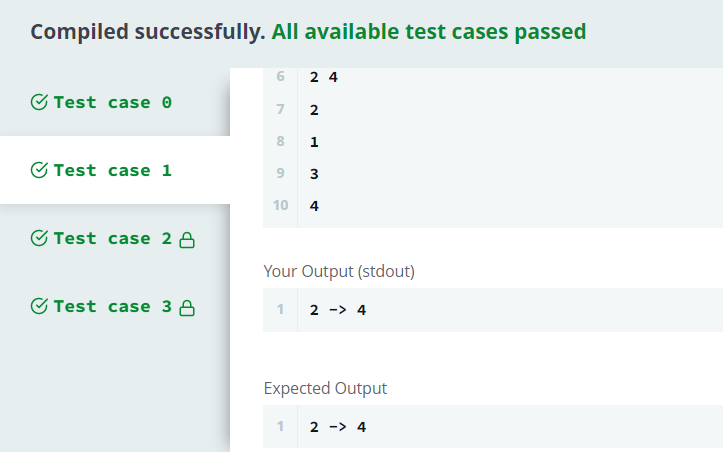
\includegraphics[width=5in]{images/admatrix.png}\\ 
\newpage
\subsection{Depth First Search}
\subsubsection{Algorithm}
\hline 
\vspace{0.1cm}
\hspace{0.5cm}Algorithm 2.b :Depth First Search
\vspace{0.1cm}
\hline

\begin{lstlisting}[label={list:first}]
  Declare a structure AdjacencyMatrix with mat[size][size] as member
  with size =10
  START OF FUNCTION insert_to_graph(AdjacencyMatrix*g,int parent,int value)
    g->mat[parent][value] =1
    g->mat[value][parent] =1
  END OF FUNCITON insert_to_graph
  
  Node is a Self Referential structure with val and node* next as members 
  START OF FUNCTION DISPLAY(node* list) \\list points to first node
  While (list!=NULL)
     Print list->val
     list=list->next
  End While
  END OF FUNCTION DISPLAY
 
  START OF FUNCTION INSERT_AT_END(node* list,int val)
  Allocate memory for new node temp
  temp->val=val
  temp->next=NULL
  If(list=NULL)
     list=temp
     Return list
  Else
     first =list               
     While(list->next!=NULL)
         list=list->next
     End While
     list->next=temp
     Return first
  End If
  END OF FUNCTION INSERT_AT_END
  
  START OF FUNCTION search(node *list,data)
  While (list!=NULL and list->val!=data)
     list=list->next
  End While
  If(list=NULL)
     return 1
  End If
  return 0
  END OF FUNCTION search
  
  Declare self referential structure Stack with data and next (which points 
  to the Stack) as members
  START OF FUNCTION push(Stack * top, int data)
  Allocate memory for ptr
  ptr->data=data
  ptr->next=top
  top=ptr
  END OF FUNCTION push
 
  START OF FUNCTION pop(Stack * top)
  If(top!=NULL)
     ptr=top
     top=top->next
     Deallocate memory for ptr
  End If
  END OF FUNCTION pop
  
  START OF FUNCTION dfs(AdjacencyMatrix*g,int startnode)
  visit=NULL
  v=startnode
  push(top,v)
  While(top!=NULL)
      v=pop(top)
      If(search(visit, v)==1)
          visit=insertAtEnd(visit,v)
          For i from 0 to size-1
              If(g->mat[v][i]==1)
                  push(top2,i)
              EndIf
          End For   
          While(top2)
              push(top,pop(top2))
          End While
      End If
  End While
  display(visit)
  END OF FUNCTION dfs
  
  START OF MAIN FUNCTION
  Allocate memory for g
  Input no. of edges n
  For i from 0 to n-1
      Input nodes a,b
      insert_to_graph(g, a,b)
  End For
  Input startnode sn
  dfs(g,sn)
  END OF MAIN FUNCTION
\end{lstlisting}
\hline


\subsubsection{Code}

\begin{lstlisting}[language=C,showstringspaces=false]
#include <math.h>
#include <stdio.h>
#include <string.h>
#include <stdlib.h>
#include <assert.h>
#include <limits.h>
#include <stdbool.h>
typedef struct AdjacencyMatrix
{
    int mat[10][10];
}AdjacencyMatrix;
AdjacencyMatrix *g;
void insert_to_graph(AdjacencyMatrix * g,int parent,int value)
{
    g->mat[parent][value] =1;
    g->mat[value][parent] =1;
}

typedef struct Stack
{
    int data;
    struct Stack* next;
}Stack;
Stack* top=NULL,*top2=NULL;

typedef struct node{
    int val;
    struct node *next;
}node;

void display(node* list){
    while(list!=NULL){
       printf("%d ",list->val);
       list=list->next;
    }
}
node* insertAtEnd(node* list,int val){
    node* temp;
    temp=(node*)malloc(sizeof(node));
    temp->val=val;
    temp->next=NULL;
    if(list==NULL)
    {
        list=temp;
        return list;
    }
    else
    {
        node*first =list;
        while(list->next!=NULL)
            list=list->next;
        list->next=temp;
        return first;
    }
}
int search(node *list,int data){
    while(list && list->val!=data){
        list=list->next;
    }
    if (list==NULL)
      return 1;
    else return 0;
}
void push(Stack**top,int data)
{
    Stack* ptr;
    ptr=(Stack*)malloc(sizeof(Stack));
    ptr->data=data;
    ptr->next=*top;
    *top=ptr;
}

int pop(Stack**top)
{
    int item;
    Stack*ptr=*top;
    item=(*top)->data;
    (*top)=(*top)->next;
    free(ptr);
    return item;
}
void dfs(AdjacencyMatrix*g,int startnode)
{
    node *visit=NULL;
    int v=startnode;
    push(&top,v);
    AdjacencyMatrix*ptr;
    while(top!=NULL){
        v=pop(&top);
        if(search(visit, v)==1){
           visit=insertAtEnd(visit,v);
           for(int i=0;i<10;i++){
               if(g->mat[v][i]==1)
                push(&top2,i);
           }
           while(top2){
               push(&top,pop(&top2));
           }
        }
    }
    display(visit);
}
int main() {
    AdjacencyMatrix * g = (AdjacencyMatrix *)malloc(sizeof(AdjacencyMatrix));
    int n,a,b,sn;
    scanf("%d",&n);
    for(int i=0;i<n;i++){
        scanf("%d %d",&a,&b);
        insert_to_graph(g, a,b);
    }
    scanf("%d",&sn);
    dfs(g,sn);
    return 0;
}

\end{lstlisting}

\subsubsection{Sample output}
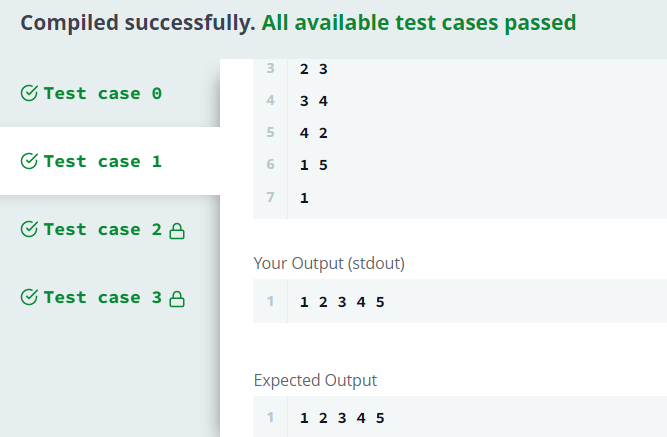
\includegraphics[width=5in]{images/dfs1.png}
\newpage
\subsection{Breadth First Search}
\subsubsection{Algorithm}
\hline 
\vspace{0.1cm}
\hspace{0.5cm}Algorithm 2.c :Breadth First Search
\vspace{0.1cm}
\hline

\begin{lstlisting}[label={list:first}]
  Declare a structure AdjacencyMatrix with mat[size][size] as member
  with size =10
  START OF FUNCTION insert_to_graph(AdjacencyMatrix*g,int parent,int value)
    g->mat[parent][value] =1
    g->mat[value][parent] =1
  END OF FUNCITON insert_to_graph
  
  Node is a Self Referential structure with val and node* next as members 
  START OF FUNCTION display(node* list) \\list points to first node
  While (list!=NULL)
     Print list->val
     list=list->next
  End While
  END OF FUNCTION display
 
  START OF FUNCTION insert_at_end(node* list,int val)
  Allocate memory for new node temp
  temp->val=val
  temp->next=NULL
  If(list=NULL)
     list=temp
     Return list
  Else
     first =list               
     While(list->next!=NULL)
         list=list->next
     End While
     list->next=temp
     Return first
  End If
  END OF FUNCTION insert_at_end
  
  START OF FUNCTION search(node *list,data)
  While (list!=NULL and list->val!=data)
     list=list->next
  End While
  If(list=NULL)
     return 1
  End If
  return 0
  END OF FUNCTION search
  
  queue is a self referential structure with front,rear and queue*link
  as members
  front=rear=NULL
  START OF FUNCTION enqueue(int k)
  If(front==NULL)
     Allocate memory for rear
     front=rear
     rear->data=k
     rear->link=NULL
  Else
     temp=rear
     Allocate memory for ptr
     ptr->data=k
     rear=ptr
     temp->link=rear
     rear->link=NULL
  End if
  END OF FUNCTION enqueue

  START OF FUNCTION dequeue()
  ptr=front
  item=ptr->data
  front=ptr->link
  Deallocate memory for ptr
  Return item
  END OF FUNCTION dequeue

  START OF FUNCTION is_empty()
  If(front==NULL)
      Return 1
  Else
      Return 0
  End if
  END OF FUNCTION is_empty
  
  START OF FUNCTION bfs(AdjacencyMatrix*g,int startnode)
  visit=NULL
  v=startnode
  enqueue(v)
  While(is_empty!=0)
      v=dequeue()
      If(search(visit, v)==1)
          visit=insertAtEnd(visit,v)
          For i from 0 to size-1
              If(g->mat[v][i]==1)
                  enqueue(i)
              EndIf
          End For   
      End If
  End While
  display(visit)
  END OF FUNCTION bfs
  
  START OF MAIN FUNCTION
  Allocate memory for g
  Input no. of edges n
  For i from 0 to n-1
      Input nodes a,b
      insert_to_graph(g, a,b)
  End For
  Input startnode sn
  bfs(g,sn)
  END OF MAIN FUNCTION
\end{lstlisting}
\hline


\subsubsection{Code}

\begin{lstlisting}[language=C,showstringspaces=false]

#include <math.h>
#include <stdio.h>
#include <string.h>
#include <stdlib.h>
#include <assert.h>
#include <limits.h>
#include <stdbool.h>
typedef struct AdjacencyMatrix
{
    int mat[10][10];
}AdjacencyMatrix;
AdjacencyMatrix *g;

typedef struct node{
    int val;
    struct node *next;
}node;

typedef struct queue{
    int data;
    struct queue* link;
}queue;
queue* rear=NULL,*front=NULL;

void insert_to_graph(AdjacencyMatrix * g,int parent,int value)
{
    g->mat[parent][value] =1;
    g->mat[value][parent] =1;
}

void enqueue(int k){
    if(front==NULL){
        rear=(queue*)malloc(sizeof(queue));
        front=rear;
        rear->data=k;
        rear->link=NULL;
    }
    else{
        queue*temp=rear;
        queue *ptr=malloc(sizeof(queue));
        ptr->data=k;
        rear=ptr;
        temp->link=rear;
        rear->link=NULL;
    }
}

int dequeue(){
    queue*ptr=front;
    int item=ptr->data;
    front=ptr->link;
    free(ptr);
    return item;
}
int is_empty(){
    if(front==NULL)
      return 1;
    return 0;
}
void display(node* list){
    while(list!=NULL){
       printf("%d ",list->val);
       list=list->next;
    }
}
node* insertAtEnd(node* list,int val){
    node* temp;
    temp=(node*)malloc(sizeof(node));
    temp->val=val;
    temp->next=NULL;
    if(list==NULL)
    {
        list=temp;
        return list;
    }
    else
    {
        node*first =list;
        while(list->next!=NULL)
            list=list->next;
        list->next=temp;
        return first;
    }
}
int search(node *list,int data){
    while(list && list->val!=data){
        list=list->next;
    }
    if (list==NULL)
      return 1;
    else return 0;
}


void bfs(AdjacencyMatrix*g,int startnode){
    node *visit=NULL;
    int v=startnode;
    enqueue(v);
    AdjacencyMatrix*ptr;
    while(is_empty()==0){
        v=dequeue();
        if(search(visit, v)==1){
           visit=insertAtEnd(visit,v);
           for(int i=0;i<10;i++){
               if(g->mat[v][i]==1)
                  enqueue(i);
           }
        }
    }
    display(visit);
}

int main() {
    AdjacencyMatrix * g = (AdjacencyMatrix *)malloc(sizeof(AdjacencyMatrix));
    int n,a,b,sn;
    scanf("%d",&n);
    for(int i=0;i<n;i++){
        scanf("%d %d",&a,&b);
        insert_to_graph(g, a,b);
    }
    scanf("%d",&sn);
    bfs(g,sn);
    return 0;
}

\end{lstlisting}

\subsubsection{Sample output}
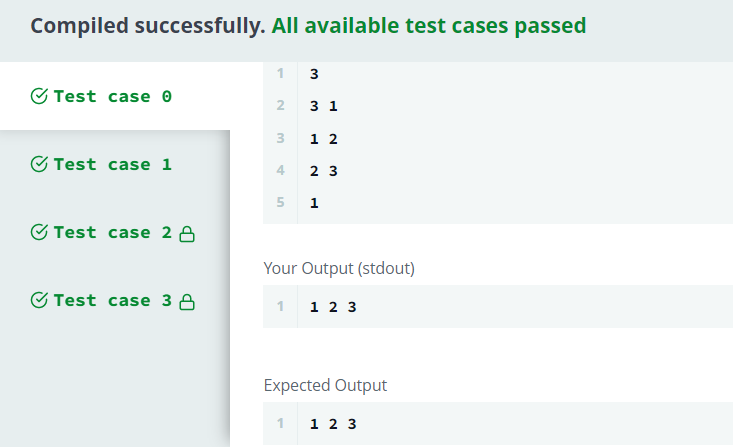
\includegraphics[width=5in]{bfs.png}\\ \\
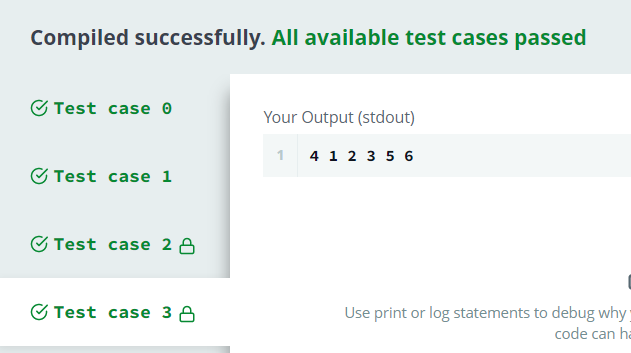
\includegraphics[width=5in]{bfs2.png}
\subsection{Result}
Program submitted and executed successfully in HackerRank Platform via user id aishwaryaaj2002
\newpage
\section{Sorting Techniques}

\subsection{Problem}
Implement following sorting techniques\\
a. Heap Sort\\
b. Merge Sort\\
c. Quick Sort
\subsection{Heap Sort}
\subsubsection{Algorithms}
\hline 
\vspace{0.1cm}
\hspace{0.5cm}Algorithm 3.a :Heap Sort Algorithm
\vspace{0.1cm}
\hline

\begin{lstlisting}[label={list:first}]
  START OF FUNCTON insert(int* ar,int n,int item)
  n=n+1
  p = n
  While (p > 1) 
      par = p / 2
      If (item <= ar[par]) 
         ar[p] = item
         return
      EndIf
      ar[p] = ar[par]
      p = par
  End While
  ar[1] = item
  END OF FUNCTION insert
  
  START OF FUNCTION delete(int*ar,int n,int item)
  item=ar[1]
  last=ar[n]
  n=n-1
  Set p=1,left=2,right=3
  While(right<=n)
      If(last>=ar[left] and last>=ar[right])
         ar[p]=last
         return
      EndIf  
      If(ar[right]<=ar[left])
         ar[p]=ar[left]
         p=left
      Else
         ar[p]=ar[right]
         p=right
        
        left=2*p
        right=left+1
    
    if(left==n and last<ar[left])
        ar[p]=ar[left]
        p=left
    
    ar[p]=last
  END OF FUNCTION delete
  
  START OF FUNCTION heap_sort(int* ar,int n)
  For i from 0 to n-1
      insert(ar, i, ar[i + 1])
  End For 
  While(n>1)
      item=ar[1]
      delete(ar, n, item)
      n=n-1
      ar[n+1]=item
  End While
  END OF FUNCTION heap_sort
  
  START OF MAIN FUNCTION
  Input no. of elements n 
  For i from 0 to n-1 
     Input ar[i]
  heap_sort(ar,0,n-1)
  For i from 0 to n-1 
     Print ar[i]
  END OF MAIN FUNCTION
\end{lstlisting}
\hline
\subsubsection{Code}
\begin{lstlisting}[language=C,showstringspaces=false]

#include <math.h>
#include <stdio.h>
#include <string.h>
#include <stdlib.h>
#include <assert.h>
#include <limits.h>
#include <stdbool.h>

void insert(int* ar,int n,int item){
    n++;
    int p = n;
    while (p > 1) {
        int par = p / 2;
        if (item <= ar[par]) {
            ar[p] = item;
            return;
        }
        ar[p] = ar[par];
        p = par;
    }
    ar[1] = item;
}
void delete(int*ar,int n,int item){
    item=ar[1];
    int last=ar[n];
    n--;
    int p=1,left=2,right=3;
    while(right<=n){
        if(last>=ar[left] && last>=ar[right]){
            ar[p]=last;
            return;
        }
        if(ar[right]<=ar[left]){
            ar[p]=ar[left];
            p=left;
        }
        else{
            ar[p]=ar[right];
            p=right;
        }
        left=2*p;
        right=left+1;
    }
    if(left==n && last<ar[left]){
        ar[p]=ar[left];
        p=left;
    }
    ar[p]=last;
}
void heap_sort(int* ar,int n){
    for (int i = 0; i < n; i++)
        insert(ar, i, ar[i + 1]);
    int item;
    while(n>1){
        item=ar[1];
        delete(ar, n, item);
        n--;
        ar[n+1]=item;
    }
}

int main() {
    int n;
    scanf("%d",&n);
    int *ar = (int*)malloc(sizeof(int)*n);
    
    for(int i = 1;i <=n; i++)
        scanf("%d",&ar[i]);
    
    heap_sort(ar,n);
    
    for(int i = 1; i <=n; i++)
        printf("%d ",ar[i]);
    return 0;
}
\end{lstlisting}

\subsubsection{Sample output}
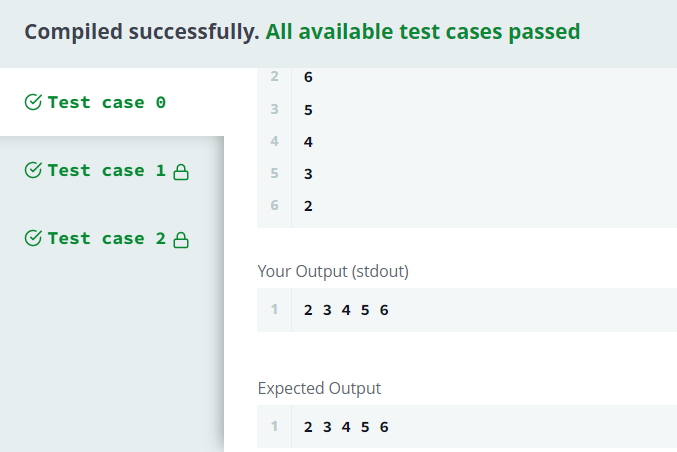
\includegraphics[width=5in]{images/mergeSort1.png}\\ \\
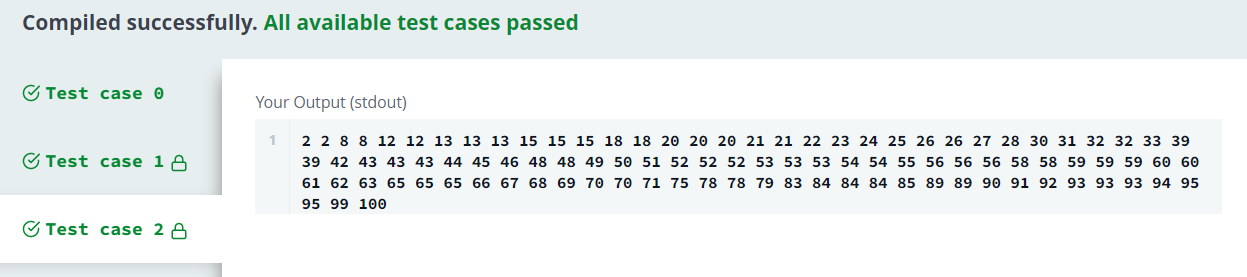
\includegraphics[width=7in]{images/mergeSort2.png}
\newpage
\subsection{Merge Sort}
\subsubsection{Algorithm}
\hline 
\vspace{0.1cm}
\hspace{0.5cm}Algorithm 3.b :Merge Sort Algorithm
\vspace{0.1cm}
\hline

\begin{lstlisting}[label={list:first}]
  
  START OF FUNCTION merge(int* ar,int l,int mid,int r){
    Set i=l,j=mid+1,k=0
    While(i<=mid and j<=r)
        If(ar[i]<=ar[j])
            c[k]=ar[i]
            k=k+1
            i=i+1
        Else
           c[k]=ar[j]
           k=k+1
           j=j+1
        EndIf
    End While
    If(i>mid and j<=r)
        For m from j to r-1
           c[k]=ar[m]
           k=k+1
        End For
    Else If(i<=mid and j>r)
        For m from i to mid
          c[k]=ar[m]
          k=k+1
        End For
    EndIf
    For m from 0 to k
      ar[l]=c[m]
      l=l+1
    End For
  END OF FUNCTION merge
  
  START OF FUNCTION merge_sort(int* ar,int l,int r)    
    If(l<r)
        mid=(l+r)/2
        merge_sort(ar,l, mid)
        merge_sort(ar,mid+1, r)
        merge(ar,l,mid,r)
    EndIf
  END OF FUNCTION merge_sort
  
  START OF MAIN FUNCTION
  Input no. of elements n 
  For i from 0 to n-1 
     Input ar[i]
  merge_sort(ar,0,n-1)
  For i from 0 to n-1 
     Print ar[i]
  END OF MAIN FUNCTION
\end{lstlisting}
\hline


\subsubsection{Code}

\begin{lstlisting}[language=C,showstringspaces=false]

#include <math.h>
#include <stdio.h>
#include <string.h>
#include <stdlib.h>
#include <assert.h>
#include <limits.h>
#include <stdbool.h>

void merge(int* ar,int l,int mid,int r){
    int i=l,j=mid+1,k=0,c[r-l+1];
    while(i<=mid && j<=r){
        if(ar[i]<=ar[j])
            c[k++]=ar[i++];
        else
          c[k++]=ar[j++];
    }
    if(i>mid && j<=r){
        for(int m=j;m<=r;m++)
          c[k++]=ar[m];
    }
    else if(i<=mid && j>r){
        for(int m=i;m<=mid;m++)
          c[k++]=ar[m];
    }
    for(int m=0;m<k;m++)
      ar[l++]=c[m];
}

void merge_sort(int* ar,int l,int r){
    if(l<r){
        int mid=(l+r)/2;
        merge_sort(ar,l, mid);
        merge_sort(ar,mid+1, r);
        merge(ar,l,mid,r);
    }
}

int main() {
    int n;
    scanf("%d",&n);
    int *ar = (int*)malloc(sizeof(int)*n);

    for(int i = 0;i < n; i++)
        scanf("%d",&ar[i]);

    merge_sort(ar,0,n-1);

    for(int i = 0; i < n; i++)
        printf("%d ",ar[i]);
    return 0;
}


\end{lstlisting}

\subsubsection{Sample output}
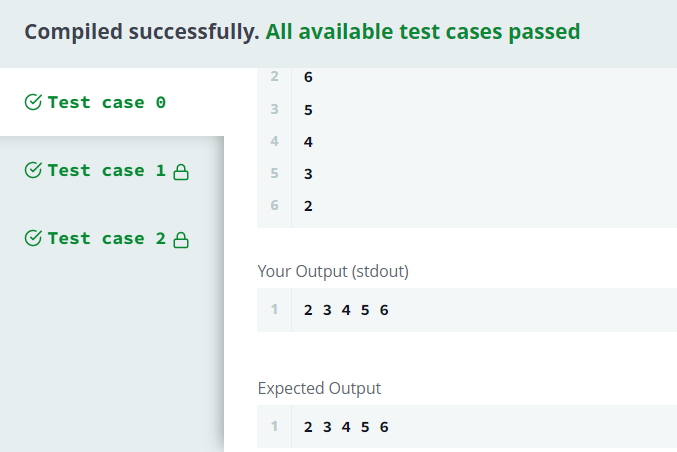
\includegraphics[width=5in]{images/mergeSort1.png}\\ \\
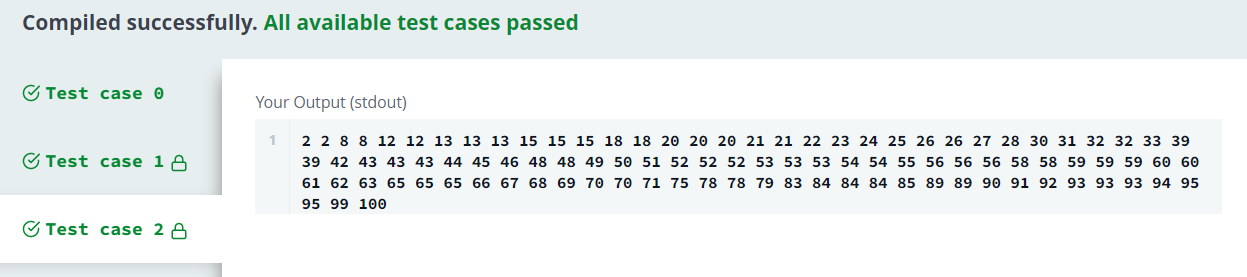
\includegraphics[width=7in]{images/mergeSort2.png}
\newpage
\subsection{Quick Sort}
\subsubsection{Algorithm}
\hline 
\vspace{0.1cm}
\hspace{0.5cm}Algorithm 3.c :Quick Sort Algorithm
\vspace{0.1cm}
\hline

\begin{lstlisting}[label={list:first}]
  Declare structure stack s with array op[Max_size] and top as variables
  START OF FUNCTION partition(int *ar,int left ,int right)   
    loc=left
    While(left<right)
        While(ar[loc]<=ar[right] and loc<right )
            right=right-1
        End While
        If(ar[loc]>ar[right])
            temp=ar[loc]
            ar[loc]=ar[right]
            ar[right]=temp
            loc=right
        End If
        While(ar[loc]>=ar[left] and loc>left )
            left=left+1
        End While
        If(ar[loc]<ar[left])
            temp=ar[loc]
            ar[loc]=ar[left]
            ar[left]=temp
            loc=left
        EndIf
    End While
    return loc
  END OF FUNCTION partition
  
  START OF FUNCTION quick_sort(int* ar,int first,int n){
    If(first<n)
        int loc=partition(ar,first,n)
        quick_sort(ar,first,loc-1)
        quick_sort(ar, loc+1,n)
    EndIf
  END OF FUNCTION quick_sort
 
  START OF MAIN FUNCTION
  Input no. of elements n 
  For i from 0 to n-1 
     Input ar[i]
  quick_sort(ar,0,n-1)
  For i from 0 to n-1 
     Print ar[i]
  END OF MAIN FUNCTION
\end{lstlisting}
\hline


\subsubsection{Code}

\begin{lstlisting}[language=C,showstringspaces=false]

#include <math.h>
#include <stdio.h>
#include <string.h>
#include <stdlib.h>
#include <assert.h>
#include <limits.h>
#include <stdbool.h>

int partition(int *ar,int left ,int right){
    int loc=left;
    while(left<right){
        while(ar[loc]<=ar[right] && loc<right ){
            right--;
        }
        if(ar[loc]>ar[right]){
            int temp=ar[loc];
            ar[loc]=ar[right];
            ar[right]=temp;
            loc=right;
        }
        while(ar[loc]>=ar[left] && loc>left ){
            left++;
        }
        if(ar[loc]<ar[left]){
            int temp=ar[loc];
            ar[loc]=ar[left];
            ar[left]=temp;
            loc=left;
        }
    }
    return loc;
}

void quick_sort(int* ar,int first,int n){
    if(first<n){
        int loc=partition(ar,first,n);
        quick_sort(ar,first,loc-1);
        quick_sort(ar, loc+1,n);
    }
}

int main() {
    int n;
    scanf("%d",&n);
    int *ar = (int*)malloc(sizeof(int)*n);

    for(int i = 0;i < n; i++)
        scanf("%d",&ar[i]);

    quick_sort(ar,0,n-1);

    for(int i = 0; i < n; i++)
        printf("%d ",ar[i]);
    return 0;
}

\end{lstlisting}

\subsubsection{Sample output}
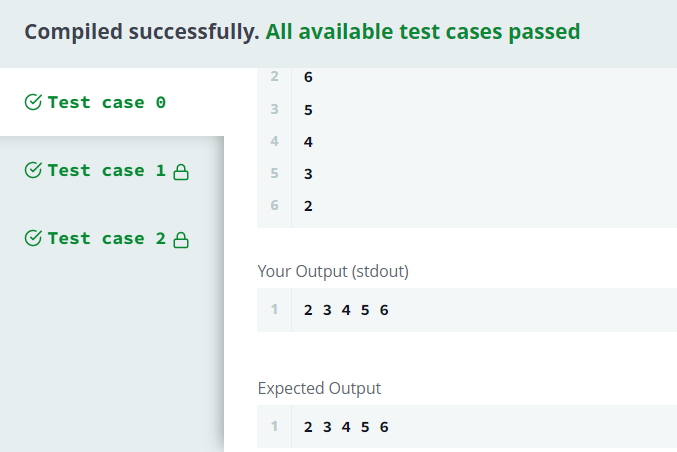
\includegraphics[width=5in]{images/mergeSort1.png}\\ \\
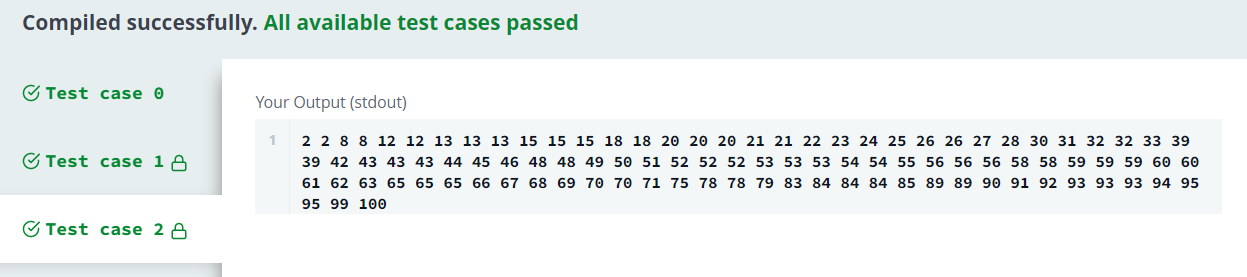
\includegraphics[width=7in]{images/mergeSort2.png}
\subsection{Result}
Program submitted and executed successfully in HackerRank Platform via user id aishwaryaaj2002
\newpage
\section{Hash Table using Chaining Method}

\subsection{Problem}
Implement a Hash table using the Chaining method. Let the size of the hash table be 10 so
that the index varies from 0 to 9.
\subsection{Algorithm}
\hline 
\vspace{0.1cm}
\hspace{0.5 cm}Algorithm 4:Hash Table using Chaining Method
\vspace{0.1cm}
\hline

\begin{lstlisting}[label={list:first}]
  Table is a self-referential structure with value and Table*link as members
  HashTable t is an array of Table h with size =10
  
  START OF FUNCTION hashingFunction(int value)
  return value%10
  END OF FUNCTION hashingFunction
  
  START OF FUNCTION insert_to_table(HashTable * t,int value)
  k=hashingFunction(value)
  If(t->h[k]==NULL)
      Allocate memory for t->h[k]
      t->h[k]->value=k
  EndIf
  ptr=t->h[k]
  Allocate memory for node
  node->value=value
  node->link=NULL
  While(ptr->link!=NULL)
       ptr=ptr->link
  End While
  ptr->link=node
  END OF FUNCTION insert_to_table
  
  START OF FUNCTION print_table(HashTable * t)
  Set flag=0
  For i from 0 to size-1
     If(t->h[i])
        flag=1
        ptr=t->h[i]
        Print i ->
        While(ptr->link!=NULL)
            Print ptr->link->value
            ptr=ptr->link
        End While
        Print "\n"
     EndIf
  End For
  If(flag==0)
      Print "Hashtable Empty !"
  End If
  END OF FUNCTION print_table
  
  START OF FUNCTION does_exist(HashTable * t, int value)
  k=hashingFunction(value)
  If(t->h[k])
     ptr=t->h[k]->link
         While(ptr!=NULL)
             If(ptr->value==value)
                return 1
             EndIf
             ptr=ptr->link
         End While
  EndIf
  return 0
  END OF FUNCTION does_exist
  
  START OF MAIN FUNCTION
  Allocate memory for hashtable t
  While(1)
    Input choice
    Switch(choice)
        Case1 : Input value
                insert_to_table(t,value)
                break
        Case 2: Input value
                exists = does_exist(t,value)
                Print exists
                break
        Case 3: print_table(t)
                break
        Case 4: return 0
    End Switch-Case
  End While
  END OF MAIN FUNCTION
\end{lstlisting}
\hline


\subsection{Code}

\begin{lstlisting}[language=C,showstringspaces=false]

#include <math.h>
#include <stdio.h>
#include <string.h>
#include <stdlib.h>
#include <assert.h>
#include <limits.h>
#include <stdbool.h>

typedef struct Table
{
   int value;
   struct Table *link;
}Table;

typedef struct HashTable
{
   Table *h[10];
}HashTable;

int hashingFunction(int value)
{
    return value%10;
}

void insert_to_table(HashTable * t,int value)
{
    int k=hashingFunction(value);
    if(t->h[k]==NULL){
        t->h[k]=(Table *)malloc(sizeof(Table));
        t->h[k]->value=k;
    }
    Table *ptr=t->h[k];
    Table *node=(Table*)malloc(sizeof(Table));
    node->value=value;
    node->link=NULL;
    while(ptr->link!=NULL)
       ptr=ptr->link;
    ptr->link=node;
}

void print_table(HashTable * t)
{
    int i,flag=0;
    for(i=0;i<10;i++){
        if(t->h[i]){
            flag=1;
            Table *ptr=t->h[i];
            printf("%d ->",i);
            while(ptr->link){
              printf(" %d",ptr->link->value);
              ptr=ptr->link;
            }
            printf("\n");
        }
    }
    if(flag==0)
      printf("Hashtable Empty !\n");
}

int does_exist(HashTable * t, int value)
{
    int k=hashingFunction(value);
    if(t->h[k]){
        Table *ptr=t->h[k]->link;
            while(ptr){
              if(ptr->value==value)
                return 1;
              ptr=ptr->link;
            }
    }
    return 0;
}

int main() {
    HashTable * t = (HashTable *)malloc(sizeof(HashTable));
    while(1)
    {
        int choice;
        scanf("%d",&choice);
        switch(choice)
        {
            case 1:
            {
                int value;
                scanf("%d",&value);
                insert_to_table(t,value);
            }
            break;

            case 2:
            {
                int value;
                scanf("%d",&value);
                int exists = does_exist(t,value);
                printf("%d\n",exists);
            }
            break;

            case 3:
            {
                print_table(t);
            }
            break;

            case 4:
            {
                return 0;
            }
        }
    }
    return 0;
}

\end{lstlisting}

\subsection{Sample output}
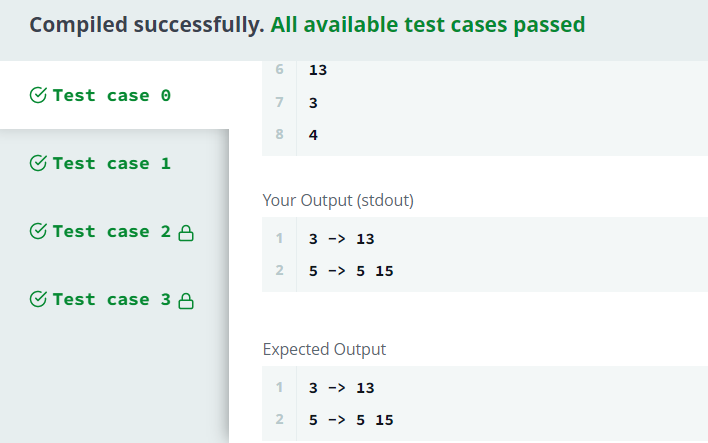
\includegraphics[width=5in]{images/htchain.png}\\ \\
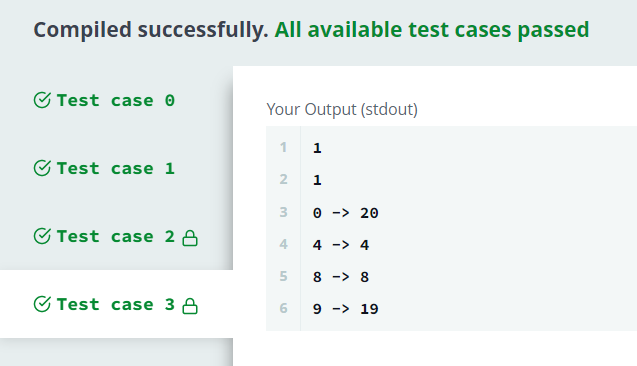
\includegraphics[width=5in]{images/htchain2.png}
\subsection{Result}
Program submitted and executed successfully in HackerRank Platform via user id aishwaryaaj2002
\newpage
\section{Hash table using Linear Probing}

\subsection{Problem}
Implement a Hash table that uses Linear Probing for collision resolution.
\subsection{Algorithm}
\hline 
\vspace{0.1cm}
\hspace{0.5cm}Algorithm 5:Hash table using Linear Probing algorithm
\vspace{0.1cm}
\hline
\begin{lstlisting}[label={list:first}]
  Declare HashTable ht,an array with SIZE=10 
  START OF FUNCTION hash(int val)
  return value%10
  END OF FUNCTION hash
  
  START OF FUNCTION insert(HashTable ht,int val){
  k=hash(val)
  i=k
  Do While(i!=k)
      If(ht[i]==0)
         ht[i]=val
         return
      EndIf
      i=(i+1) mod SIZE
  End Do While
  END OF FUNCTION insert
  
  START OF FUNCTION print(HashTable ht)
  For i from 0 to SIZE-1
      Print i,ht[i]
  END OF FUNCTION print
  
  START OF FUNCTION doesExist(HashTable ht,int val){
  k=hash(val)
  Set i=k
  Do While(i!=k)
      If(ht[i]==val)
          return 1
      EndIf
      i=(i+1) mod SIZE
  End Do While
  return 0
  END OF FUNCTION doesExist
  
  START OF MAIN FUNCTION
  Allocate memory for hashtable ht
  While(1)
    Input opt
    Switch(opt)
        Case1 : Input val
                insert(ht,val)
                break
        Case 2: Input val
                exists = doesExist(ht,val)
                If(exists=1)
                   Print "Exists"
                Else
                    Print "Doesn't Exist"
                EndIf
                break
        Case 3: print(ht)
                break
        Case 4: return 0
    End Switch-Case
  End While
  END OF MAIN FUNCTION
\end{lstlisting}
\hline


\subsection{Code}

\begin{lstlisting}[language=C,showstringspaces=false]

#include <math.h>
#include <stdio.h>
#include <string.h>
#include <stdlib.h>
#include <assert.h>
#include <limits.h>
#include <stdbool.h>

#define SIZE 10
typedef int* HashTable;

int hash(int val){
    return val%SIZE;
}

void insert(HashTable ht,int val){
    int k=hash(val);
    int i=k;
    do {
        if(ht[i]==0){
            ht[i]=val;
            return;
        }
        i=(i+1)%SIZE;
    }while (i!=k);
}

int doesExist(HashTable ht,int val){
    int k=hash(val),i=k;
    do {
        if(ht[i]==val){
            return 1;
        }
        i=(i+1)%SIZE;
    }while (i!=k);
    return 0;
}

void print(HashTable ht){
      for(int i=0;i<SIZE;i++)
          printf("%d %d\n",i,ht[i]);
}

int main(){
    HashTable ht = (int*)malloc(sizeof(int)*SIZE);
    int opt,val,exists;

    do{
        scanf("%d",&opt);
        switch(opt){
            case 1: scanf("%d",&val);
                    insert(ht,val);
                    break;
            case 2: scanf("%d",&val);
                    exists = doesExist(ht,val);
                    if(exists)
                        printf("Exists\n");
                    else
                        printf("Doesn't Exist\n");
                    break;
            case 3: print(ht);
                    break;
        }

    }while(opt != 4);
    return 0;
}
\end{lstlisting}

\subsection{Sample output}
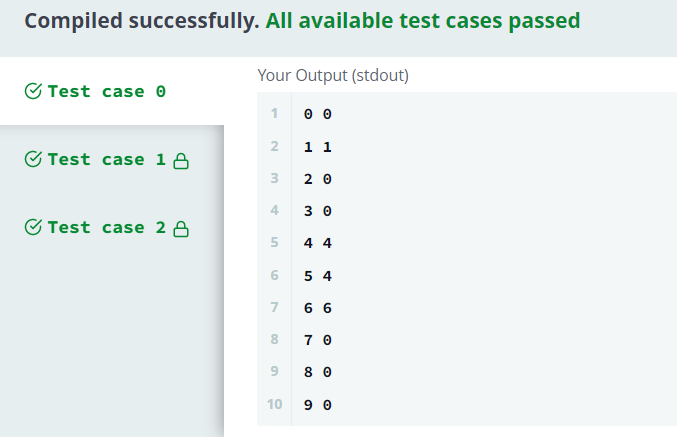
\includegraphics[width=5in]{images/hashlinear.png}
\subsection{Result}
Program submitted and executed successfully in HackerRank Platform via user id aishwaryaaj2002



\end{document}